\section{Autoencoders and Adversarial Examples}\label{sec:combining}
In this section we take a look at work that combines adversarial examples and
variational autoencoders.

\subsection{Adversarial Images for Autoencoder}
This approach \cite{tabacof2016adversarial} describes a method for creating a
distortion based on variational autoencoders: The attack consists of selecting
an original image and a target image and then feeding the network with the
original image modified by a small distortion, optimized to get the result as close
as possible to the target image (Figure
\ref{fig:adversarial_images_autoencoder}). Autoencoders reconstruct from the
latent representation, which makes it the information bottleneck, and therefore
particularly convenient to attack. The authors used the following adversarial
optimization:
    
\begin{align}
    & \min_{d} \quad \Delta(\vect{z}_{a}, \vect{z}_{t}) + C||\vect{d}|| && \\
    & s.t. \quad  
        \begin{aligned}[t]
            & L \leq \vect{x} + \vect{d} \leq U \\
            & \vect{z}_a = encoder(\vect{x} + \vect{d})
        \end{aligned}
\end{align}

\begin{figure}
	\centering
	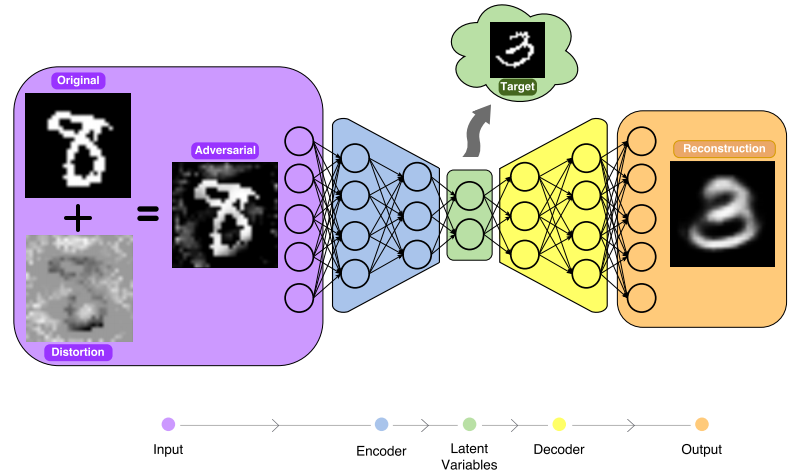
\includegraphics[width=\linewidth]{/4/adversarial_images_autoencoder}
    \caption{Adversarial attacks for autoencoders apply distortions to the input
    with the goal of having the autoencoder reconstruct another target. The
    latent representation is attacked, by attempting to match it to the target
    image's
    \cite{tabacof2016adversarial}.} 
	\label{fig:adversarial_images_autoencoder}
\end{figure}

where $\vect{d}$ is the adversarial distortion; $\vect{z}_{a}$ and
$\vect{z}_{t}$ are the latent representations of the adversarial and the target
images; $\vect{x}$ is the original image; $\vect{x} + \vect{d}$ is the
adversarial image; $L$ and $U$ are bounds on the input space; and C is the
regularizing constant that balances reaching the target and limiting the
distortion.

For variational autoencoders $\Delta$ is chosen as the the KL-divergence to
measure the difference between the two probabilty distributions. $z_{*}$
correspond to uncorrelated multivariate normal distributions with parameters
given by the encoder:

\begin{equation}
    encoder(\vect{x}) \sim \mathcal{N}\big(\vect{M}_{\theta}(\vect{x}), \vect{\Sigma}_{\theta}(\vect{x})\big)
\end{equation}

where $\vect{M}$ and $\vect{\Sigma}$ represent the mean vector, and the
covariance matrix outputted by the last layer of the encoder network; $\theta$
are the autoencoder parameters \---- learned previously by training it for its
ordinary task of reconstruction. During the entire adversarial optimization,
$\theta$ remains fixed.

Results of this experiment show that generating adversarial images for
autoencoders is a much harder task than for classifiers. If a little distortion
(comparable to those used for misleading classifiers) is applied, the
reconstruction stays almost untouched. To get reconstructions very close to the
target's, it is necessary to add heavy distortions to the input. However, by
hand-tuning the regularization parameter, it is possible to find trade-offs
where the reconstruction approaches the target's and the adversarial image will
still look like the input.

\subsection{Purify Adversarial Examples with PuVAE}
\begin{figure}
	\centering
	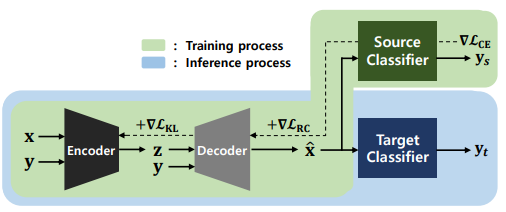
\includegraphics[width=\linewidth]{/4/puvae_1}
    \caption{Overview of the PuVAE algorithm; The green region shows the
    training process, and the blue region denotes the inference process of
    PuVAE. The dotted line represents the gradient flow during training. The
    parameters off the source classifier are not updated \cite{hwang2019puvae}.}
    
	\label{fig:puvae_1}
\end{figure}

Authors of this paper \cite{hwang2019puvae} introduced a defense mechanisms
based on variational autoencoders. They propose Purify Variational Autoencoder
(PuVAE), a method to purify adversarial examples. The proposed method eliminates
an adversarial perturbation by projecting an adversarial example on the manifold
of each class, and determines the closest projection as a purified sample.

\subsubsection{Training PuVAE}
A data set $\mathcal{X}$ is defined which contains clean samples and adversarial
examples. Similiar as explained in subsection \ref{subsec:varautoencoders} the
authors trained PuVAE by maximizing the variational lower bound associated with
a datapoint $x$ from $\mathcal{X}$. Additionally, a cross-entropy calculated
from a classifier is used as a loss function for PuVAE. The classifier, called
\textit{source} classifier $M_{s}$, learns the decision boundaries on the data
space. The trained $M_{s}$ is used to ensure that the output instance reflects
the characteristics of the classes in the dataset. The cross-entropy loss from
$M_{s}$ is as follows:

\begin{equation}
    \vect{y}_{s} = M_{s}(\hat{\vect{x}})
\end{equation}
\begin{equation}
    \mathcal{L}_{CE} = \vect{y}_{data} \log \vect{y}_{s} + (1 - \vect{y}_{data}) \log (1 - \vect{y}_s)
\end{equation}

Finally, the PuVAE is trained using stochastic gradient descent:

\begin{equation}
    \nabla(\lambda_{RC} \mathcal{L}_{RC} + \lambda_{KL} \mathcal{L}_{KL} + \lambda_{CE} \mathcal{L}_{CE})
\end{equation}

where $\mathcal{L}_{RC}$ denotes the reconstruction loss and $\mathcal{L}_{KL}$
denotes the Kullback-Leibler divergence (both described in equation \ref{vae:2})
and $\mathcal{L}_{CE}$ the loss from the $M_{s}$ classifier. Figure
\ref{fig:puvae_1} gives an overview of the training process of PuVAE.


\subsubsection{Generating Purified Samples}
During inference time, the PuVAE projects an input sample to the data manifolds
of all classes in the dataset as follows:

\begin{equation}
    \hat{\vect{x}}_{y_i} = PuVAE(x, \vect{y_{i}})
\end{equation}

where $\vect{y}_i$ denotes the i-th class label to guide the input to the
corresponding latent space, and $\hat{\vect{x}}_{y_i}$, denotes a candidate for
the purified sample. Because PuVAE only learns the distribution of $\vect{z}$
from the training data, the input is mapped to the learned latent spaces even if
adversarial examples come in. The adversarial perturbations are removed in the
projection to the latent variable.

Then, the class label $y^*$ corresponding to the closest projection is selected as follows:

\begin{equation}
    \vect{y^*} = argmin_{y_{i} \in C} D(\vect{x}, \hat{\vect{x}}_{i})
\end{equation}

where $D$ denotes a distance measure to determine the closest projection and $C$
is the set of all possible class labels. The authors used the root mean square
error as the distance measure. Therefore, the candidate generated with label
$\vect{y}^*$ is the purified sample which goes into $M_{t}$:

\begin{equation}
    \vect{x}_{purified} = \hat{\vect{x}}_{y^*}
\end{equation}

At last, the purified sample is processed by the target classifier $M_{t}$ as follows:

\begin{equation}
    \vect{y}_{t} = M_{t}(\vect{x}_{purified})
\end{equation}

The authors test the robustness of PuVAE against various attack methods. PuVAE
exihibit performances competitive with state-of-the-art defense methods, and the
inference time is approximately 130 times faster than that of Defense-GAN that
is the state-of-the art purifier model.